\documentclass[sigconf]{acmart}

\renewcommand\footnotetextcopyrightpermission[1]{} % removes footnote with conference information in first column
\pagestyle{fancy} % removes running headers

\setlength{\parskip}{0pt}
\setlength{\parsep}{0pt}
\setlength{\headsep}{0pt}
\setlength{\topskip}{0pt}
\setlength{\topmargin}{0pt}
\setlength{\topsep}{0pt}
\setlength{\partopsep}{0pt}
%\linespread{0.95}
\usepackage{mdwlist}

\usepackage{amsmath}
\fancyhead{}
\settopmatter{printacmref=false, printfolios=false}
% Copyright
\setcopyright{none}
% \setcopyright{acmcopyright}
% \setcopyright{acmlicensed}
% \setcopyright{rightsretained}
% \setcopyright{usgov}
% \setcopyright{usgovmixed}
% \setcopyright{cagov}
% \setcopyright{cagovmixed}

\settopmatter{printacmref=false} % Removes citation information below abstract
\begin{document}
\title{Minimum Edit Distance Performance for Auto-spell Correction}
\titlenote{https://github.com/feknall/spell-correction-minimum-edit-distance}
\author{Hamid Fazli Khojir}
% \authornotemark[1]
\orcid{0000-0002-6033-6564}
\affiliation{
 \institution{University of Windsor}
%   \city{Fredericton} 
%   \state{NB} 
%   \country{Canada} 
}\email{fazlikh@uwindsor.ca}

\maketitle

\section{Introduction}
Finding the similarity between two string has many applications in NLP, genetics, and etc. Since string are not like real numbers and we cannot find the similarity between two string just by simple additions and subtraction, we need to define a new term, called minimum edit distance. Minimum edit distance is defined as the minimum number of modifications (add, remove, replace) that is required to convert one string to another string. Levenshtein distance, Longest common subsequence, and Hamming distance are famous edit distances. In NLP, corpus is a collection of texts that will be used as a base for NLP tasks. Birkbeck is a relatively old corpus that can be used to extract a pair of wrong and correct words, and is publicly available.
Wordnet is a public English dictionary with almost 150,000 words that is available in many python libraries like nltk and PyDictionary. Considering those three elemnts, we want to use an statistical approach to find the correct spelling of a misspelled word. 
% In this assignment, we want to find the correct spell of a word. Since we want to use statistical analysis to do this, we need a corpus that is consisted of a pair of wrong and correct words.
\section{Motivation}
Writing is one of the main ways of communication. However, we may write a misspelled word because of many different reasons. The main purpose of our work is to reduce these kinds of mistakes by suggesting the correct spelling of a misspelled word.
\section{Problem Definition}
Given a dictionary $\mathcal{D}$, a corpus of a pair of misspelled and correct tokens $\mathcal{C}$, a pair of token ($tMisspelled$, $tCorrect$) $\in$ $\mathcal{C}$, top-$k$ least distance of token $tMisspelled$ is desired.
Next, based on the $tCorrect$ and $x$ $\in$ top-$k$, average of $s$@$k$  needs to be calculated for $k$ $\in$ $\{1, 5, 10\}$
\subsection{Example}
For misspelled word 'prepearing', top-10 similar words are ('rehearing', 2), ('repeating', 2), ('pampering', 3), ('preceding', 3), ('propelling', 3), ('prospering', 3), ('rearing', 3), ('releasing', 3), ('repelling', 3), ('revealing', 3). The number in parentheses is the minimum edit distance according to Levenshtein distance.
\section{Experiment}
\subsection{Datasets}
Birkbeck dataset is consisted of many different files for different purposes. After considering all of those files, we have decided to use EXAMSDAT as our corpus because of two main reasons. Firstly, this file has more misspelled words compared to other files. Secondly, we need to know the correct spelling of the misspelled word to evaluate s@k. EXAMSDAT has 12,231 pairs of words, and 6,817 pairs of unique words. We have removed duplicated words for our experiment.
% Figure~\ref{fig:birkbeck} shows a comparison between all words and unique words in EXAMSDAT.
% \begin{figure}[!htb]
% \centerline{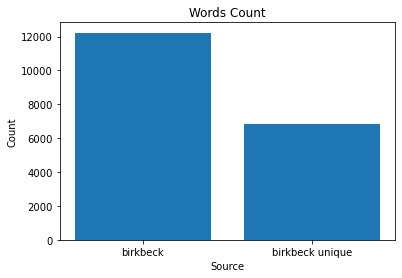
\includegraphics[width=14pc]{birkbeck.png}}
% \caption{Solving a maze by using the wall follower algorithm}
% \label{fig:birkbeck}
% \end{figure}
\subsection{Results}
As Figure~\ref{fig:success_at_k} shows, for k equal to 1, 5, and 10, s@k is 0.285, 0.473, 0.517, respectively.
\begin{figure}[!htb]
\centerline{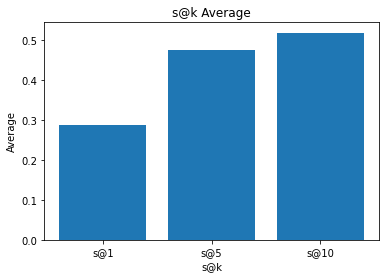
\includegraphics[width=14pc]{success_at_k.png}}
\caption{Success at K}
\label{fig:success_at_k}
\end{figure}
Calculating the edit distance between each misspelled word and all words of dictionary is time consuming. In order to handle this problem, we have used 200 different processes. Therefore, the whole process of finding similar words and calculating s@k takes almost 10 minutes when using Cedar cluster of Sharcnet. Figure~\ref{fig:job_seconds} shows the life time of each process.
\begin{figure}[!htb]
\centerline{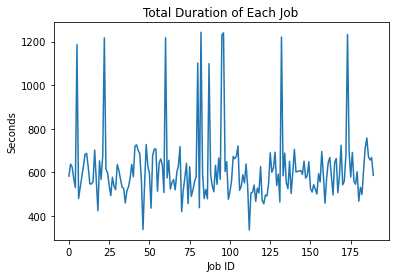
\includegraphics[width=16pc]{job_seconds.png}}
\caption{Solving a maze by using the wall follower algorithm}
\label{fig:job_seconds}
\end{figure}

\section{Conclusion}
In this work, we successfully calculated average s@k. As we expected, the probability of success will increase by increasing k. Additionally, the difference between s@1 and s@5 is much greater than s@5 and s@10, which shows that the relation between success and k is not linear.
% \bibliographystyle{ACM-Reference-Format}
% \bibliography{bibliography.bib} 

\end{document}

